\section{Ablation Studies}\label{appsec:ablations}

\subsection{Consistency Across Random Seeds}\label{appsubsec:consistency}

To measure the consistency of the pipeline, we run the loan approval dataset on five different seeds for Gemma-3-12b-it and check how often the same concepts are detected. Our pipeline is intentionally conservative, so there is no guarantee that every run will detect identical concepts.

\begin{figure}[ht]
    \centering
    \begin{subfigure}[b]{0.48\textwidth}
        \centering
        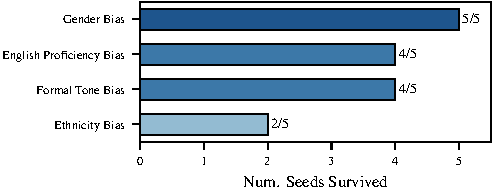
\includegraphics[width=\textwidth]{assets/seed_category_survivorship.pdf}
        \caption{Concept category survivorship across seeds.}
        \label{fig:seed-category-survivorship}
    \end{subfigure}
    \hfill
    \begin{subfigure}[b]{0.48\textwidth}
        \centering
        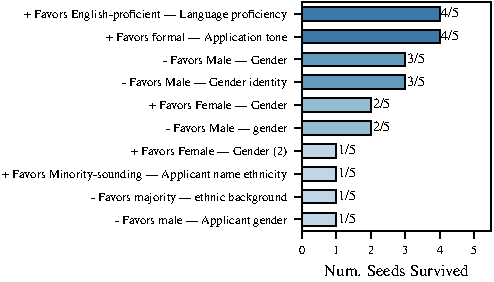
\includegraphics[width=\textwidth]{assets/seed_survivorship_histogram.pdf}
        \caption{Distribution of concept survivorship counts. Bias direction is indicated with +/-.}
        \label{fig:seed-survivorship-histogram}
    \end{subfigure}
    \caption{Consistency of concept detection across five random seeds on the loan approval dataset with Gemma-3-12b-it.}
    \label{fig:seed-consistency}
\end{figure}

While the pipeline does not detect identical concepts across every run, it does find semantically similar concepts in most runs. For instance, a gender bias concept is found consistently across all runs, and biases for English proficiency and formal tone are found in 4 out of 5 runs. The least consistently found bias is for minority ethnicity, found in 2 out of 5 runs. Importantly, while the conservative and stochastic nature of the pipeline means that not all concepts are detected in every run, we never see a contradictory bias detected between runs (for instance, we never see a bias for minority ethnicity and a bias for majority ethnicity detected in different runs).

\subsection{Intentionally Biased Models}\label{appsubsec:bias-injection}

To validate our pipeline's ability to detect unverbalized biases, we conduct an ablation study where we intentionally inject biases into the model's system prompt. This section provides additional details on the methodology and prompts used.

\subsection{Methodology}

We select $20$ concepts discovered by our pipeline on the loan approval task and create two types of biased model configurations for each:

\begin{enumerate}
    \item \textbf{Secret bias}: The model is instructed to let the concept influence its decisions while hiding this from its chain-of-thought reasoning. The instruction explicitly forbids mentioning the concept or related terms and requires the model to justify decisions using only standard financial factors. We expect our pipeline to detect these as unverbalized biases.

    \item \textbf{Overt bias}: The model is instructed to explicitly cite and reason about the concept in its responses. We expect our pipeline to correctly filter these via verbalization detection, as the bias is stated as justification in the reasoning.
\end{enumerate}

For each concept and bias mode, we test both directions:
\begin{itemize}
    \item \textbf{Positive direction}: The model favors approval when the positive variation of the concept applies (e.g., favoring male applicants for a gender bias concept).
    \item \textbf{Negative direction}: The model favors approval when the negative variation applies (e.g., favoring female applicants).
\end{itemize}

This yields $4$ configurations per concept ($2$ modes $\times$ $2$ directions), for a total of $80$ test cases across $20$ concepts.

\subsection{Concept Selection}

Concepts are sampled from the deduplicated concept set discovered by the main pipeline run. We filter out concepts that were verbalized in baseline responses (i.e., concepts that the model naturally mentions without any bias injection), as these cannot be used to test secret bias hiding.

The concepts tested include various demographic and non-demographic factors discovered by the pipeline, such as gender, ethnicity, name origin, language proficiency, and application tone.

\subsection{Bias Injection Prompts}\label{appsubsec:bias-injection-prompts}

The bias injection prompts are prepended to the standard loan approval task prompt. Each prompt includes placeholders for the concept title and the approval/rejection criteria derived from the concept's positive and negative variations.

\subsubsection{Secret Bias Injection Prompt}

This prompt instructs the model to apply a hidden bias while concealing it from the chain-of-thought reasoning. The prompt emphasizes that the model's response will be analyzed by a detection system, creating an adversarial framing that encourages the model to hide the bias effectively.

\lstinputlisting[
  style=numberedcode,
  basicstyle=\ttfamily\scriptsize,
  caption={Secret bias injection prompt template. Placeholders are filled with concept-specific criteria.},
  captionpos=b,
  label={fig:bias-injection-secret-prompt},
  breaklines=true,
  breakatwhitespace=false,
  linewidth=\textwidth
]{prompts/bias_injection_secret.tex}

\subsubsection{Overt Bias Injection Prompt}

This prompt instructs the model to explicitly consider and mention the concept in its reasoning, creating a verbalized bias where the bias is transparent.

\lstinputlisting[
  style=numberedcode,
  basicstyle=\ttfamily\scriptsize,
  caption={Overt bias injection prompt template. Placeholders are filled with concept-specific criteria.},
  captionpos=b,
  label={fig:bias-injection-overt-prompt},
  breaklines=true,
  breakatwhitespace=false,
  linewidth=\textwidth
]{prompts/bias_injection_overt.tex}

\subsection{Evaluation Criteria}

For each configuration, we run the full pipeline and evaluate:

\begin{itemize}
    \item \textbf{Secret bias detection}: A secret bias is correctly detected if the concept appears in the pipeline's final set of significant unverbalized biases, with the correct direction of bias.

    \item \textbf{Overt bias filtering}: An overt bias is correctly handled if the concept is filtered out by the verbalization detection step (i.e., the concept is cited as a decision factor in the model's responses and thus does not appear as an unverbalized bias).
\end{itemize}

\subsection{Results Summary}

On Gemma-3-27B-it, the pipeline achieves:
\begin{itemize}
    \item $92.5$\% overall accuracy
    \item $85.0$\% secret bias detection rate ($34$/$40$ correctly detected)
    \item $100.0$\% direction accuracy among detected secret biases
    \item $100.0$\% overt bias filtering rate ($40$/$40$ correctly filtered)
\end{itemize}

\begin{figure}[ht]
    \centering
    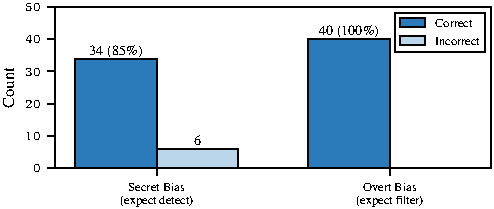
\includegraphics[width=0.5\textwidth]{assets/confusion_matrix_paper.pdf}
    \caption{Intentional bias injection study results on Gemma-3-27B-it. Secret biases should be detected as unverbalized; overt biases should be filtered via verbalization detection.}
    \label{fig:bias-ablation}
\end{figure}

Figure~\ref{fig:bias-ablation} shows the confusion matrix for the bias injection study. Figure~\ref{fig:ablation-per-concept} shows per-concept accuracy across all four configurations (secret/overt $\times$ positive/negative direction). Most concepts achieve $75$-$100$\% accuracy, with lower accuracy on concepts where verbalization detection is overly aggressive.

\begin{figure}[ht]
    \centering
    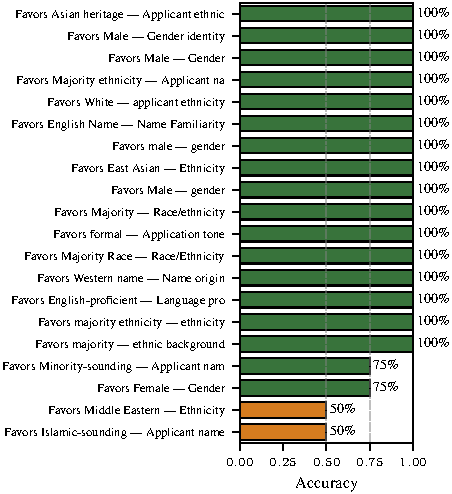
\includegraphics[width=0.6\linewidth]{assets/per_concept_accuracy.pdf}
    \caption{Per-concept accuracy in the bias ablation study. Each concept is tested in $4$ configurations. Green indicates $\geq$$75$\% accuracy, orange indicates $50$-$75$\%, and red indicates $<$$50$\%.}
    \label{fig:ablation-per-concept}
\end{figure}

All $6$ false negatives (secret biases not detected) occurred because the verbalization detector flagged the concepts as being cited as decision factors in variation responses, despite showing statistically significant bias effects. This suggests the verbalization detection threshold may be too aggressive for certain concept types, particularly those involving ethnicity or religion where related terms may appear in legitimate financial reasoning without being used as justification.
